\documentclass[dvipsnames]{beamer}
\usepackage{polyglossia}
\setdefaultlanguage{slovak}
\setbeamertemplate{caption}{\raggedright\insertcaption\par}
\setlength{\belowcaptionskip}{-13pt}
\setlength{\abovecaptionskip}{-5pt}
\setlength\intextsep{-10cm}
\definecolor{bgc}{RGB}{250,250,250}
\definecolor{tc}{RGB}{0,0,100}
\urlstyle{same}
\setbeamercolor{sectionColor}{fg=white,bg=RoyalBlue}
\setbeamercolor{background canvas}{bg=bgc,fg=white}
\setbeamercolor{normal text}{fg=tc}
\setbeamercolor{frametitle}{fg=ForestGreen}
\hypersetup{
    colorlinks=true,
    urlcolor={cyan},
    linkcolor=,
    pdfpagemode=FullScreen,
    }
\setbeamertemplate{section page}
{
    \begingroup
    \begin{beamercolorbox}[sep=12pt,center]{sectionColor}%
        \usebeamerfont{section title}\insertsection\par
    \end{beamercolorbox}
    \endgroup
}
\addtobeamertemplate{frametitle}{}{\vspace{-1.5em}}
\addtobeamertemplate{itemize subbody begin}{\scriptsize}

\title{Umenie a kultúra v 17. a 18. storočí}
\author{Adam Jenča a  Alica Jenčová, Sekunda}
\begin{document}
\begin{frame}
	\titlepage
\end{frame}
\begin{frame}
	\frametitle {Obsah}
	\begin{columns}
		\column{0.7\textwidth}
		\tableofcontents
		\column{0.3\textwidth}
		
\includegraphics{book}\\
		\vskip 2mm
		
\includegraphics[scale=0.4]{arch}\\
		\vskip 2mm
		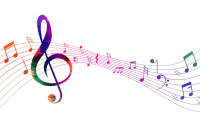
\includegraphics[scale=0.4]{music}\\
		\vskip 2mm
		
\includegraphics[scale=0.4]{palette}\\
	\end{columns}
\end{frame}
\section{Hudba}
\frame{\sectionpage}
\begin{frame}{Barok}
	\subsection{Barok}
	\begin{itemize}
		\item Začiatok hudobného novoveku
		\item Odčlenenie inštrumentálnej hudby
		\item Dôraz na polyfóniu
	\end{itemize}
	\begin{columns}
		\column{0.5\textwidth}
		
		\kern0pt
		\begin{figure}
		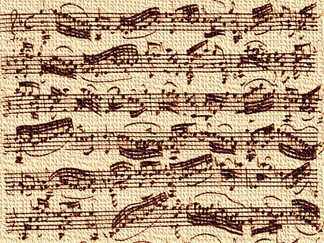
\includegraphics[scale=1.5]{baroko}
		\caption{Notový zápis z baroka}
		\end{figure}%
		
		\column{0.5\textwidth}
		\begin{figure}
			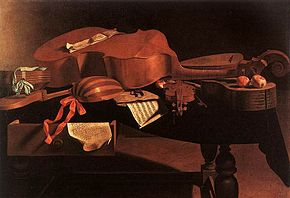
\includegraphics[scale=1.5]{in}
			\caption{Odčlenenie inštrumentálnej hudby}
		\end{figure}
	\end{columns}

\end{frame}
\begin{frame}{\small Barok / \Large Nástroje}
	\subsubsection{Nástroje}
	\begin{itemize}
		\item Najvyužívanejšie:	
		\begin{itemize}
		\item Flauta
		\item Trúbka
		\item Organ
		\item Čembalo
		\item Sláčikový orchester
		\end{itemize}
	\end{itemize}
	\begin{columns}
	\kern0pt
		\column{0.5\textwidth}
	\begin{figure}
		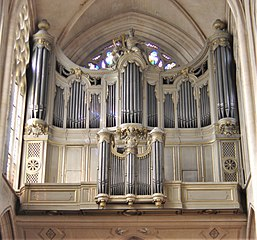
\includegraphics[scale=0.25]{organ}
		\caption{Organ}
	\end{figure}%
	\begin{figure}
		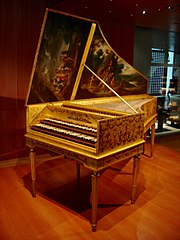
\includegraphics[scale=0.25]{cembalo}
		\caption{Čembalo}
	\end{figure}%
	\column{0.5\textwidth}
	
		\begin{figure}
			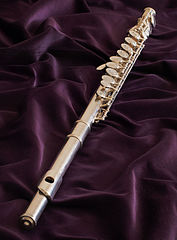
\includegraphics[scale=1.5]{flauta}
		\caption{Flauta}
	\end{figure}%
		\begin{figure}
			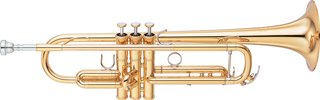
\includegraphics[scale=0.3]{truba}
		\caption{Trúbka}
	\end{figure}%

	\end{columns}
\end{frame}
\begin{frame}{\small Barok / \Large Skladatelia}
	\subsubsection{Skladatelia}
	\begin{columns}
	\column{0.5\textwidth}
	
	\begin{itemize}
		\item Raný barok
		\begin{itemize}
			\item C. Monteverdi
		\end{itemize}
		\item Vrcholný  barok
		\begin{itemize}
			\item J. S. Bach - \href{https://www.gtsforum.xyz/organ.mp3}{ukážka}
			\item G. F. Händel
			\item A. Vivaldi - \href{https://www.gtsforum.xyz/vivaldi.mp3}{ukážka}
		\end{itemize}

	\end{itemize}
	\column{0.5\textwidth}
	\begin{figure}
		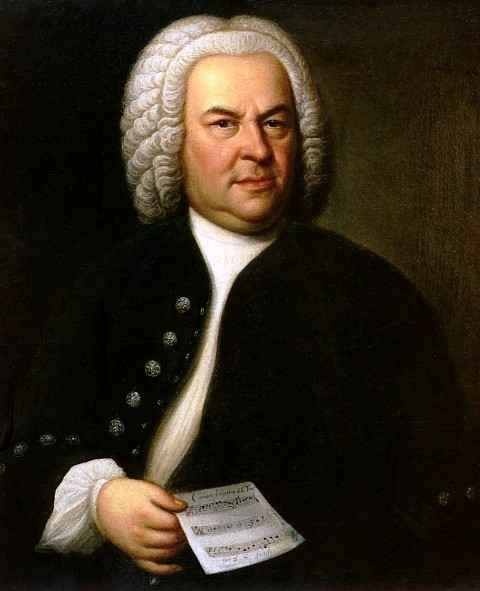
\includegraphics[scale=0.75]{bach}
		\caption{Johann Sebastian Bach}
	
	\end{figure}%
	\begin{figure}
		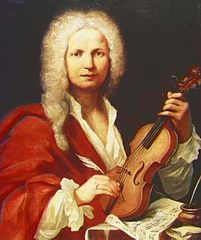
\includegraphics[scale=1.75]{vivaldi}
		\caption{Antonio Vivaldi}
	\end{figure}

	\end{columns}
\end{frame}
\begin{frame}{Klasicizmus}
	\begin{itemize}
		\item Vznik a rozvoj sonátovej formy
		\item Rozlišovanie dur/mol
		\item Vznik symfónie
		
	\end{itemize}
	\begin{figure}
		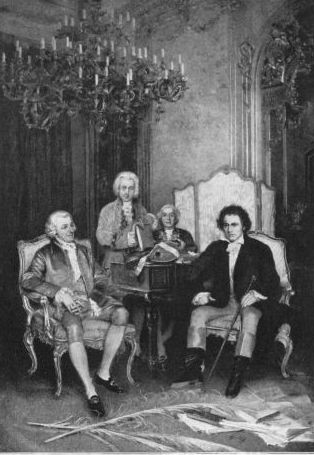
\includegraphics[scale=0.3]{klasmu}
		\caption{Najväčší skladatelia klasicizmu: Haydn, Mozart a Beethoven}
	\end{figure}
\end{frame}
\begin{frame}{\small Klasicizmus / \Large Skladatelia}
	\begin{columns}
	\column{0.7\textwidth}

	\begin{itemize}
		\item Joseph Haydn - \href{https://www.gtsforum.xyz/haydn.mp3}{ukážka}
		\item Wolfgang Amadeus Mozart - \href{https://www.gtsforum.xyz/mozart.mp3}{ukážka}
		\item Ludwig van Beethoven - \href{https://www.gtsforum.xyz/beethoven.mp3}{ukážka}
		\item Niccolò Paganini - \href{https://www.gtsforum.xyz/paganini.ogg}{ukážka}
		\item Christoph  Willibald Gluck - \href{https://www.gtsforum.xyz/gluck.ogg}{ukážka}
	\end{itemize}
	\column{0.3\textwidth}
		\begin{figure}
			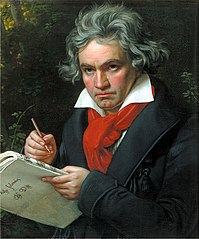
\includegraphics[scale=0.45]{beethoven}
			\caption{L. van Beethoven}
		\end{figure}
		\begin{figure}
			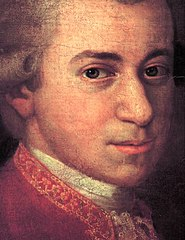
\includegraphics[scale=0.45]{mozart}
			\caption{W. A. Mozart}
		\end{figure}

	\end{columns}
\end{frame}
\section{Literatúra}
\frame{\sectionpage}

\begin{frame}{17. storočie}
	\subsection{17. storočie}	
	\begin{itemize}
		\item Renesancia -> prostredie pre nové myšlienky
		\item ,,Čo viem ?'' = skepticizmus
		\item Prechod do modernej doby + nárast významu vedy = kríza v umení
		\begin{minipage}[t]{0.4\textwidth}
		\kern0pt
		
		\begin{figure}
			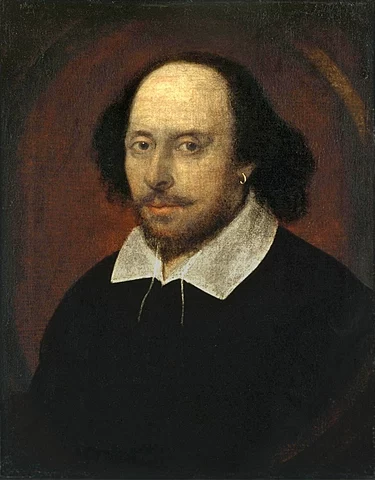
\includegraphics[scale=0.2]{pivo}
			\caption{William Shakespeare}
		\end{figure}
		\end{minipage}%
		\begin{minipage}[t]{0.6\textwidth}
		\kern0pt

		\begin{figure}
			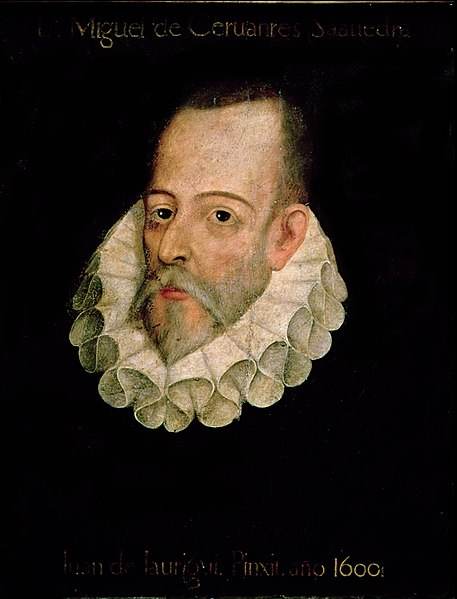
\includegraphics[scale=0.1605]{cervo}
			\caption{Miguel de Cervantes}
		\end{figure}
		\end{minipage}
	\end{itemize}
\end{frame}
\begin{frame}{\small 17. storočie / \Large Významní spisovatelia 17. storočia}
	\subsubsection{Významní spisovatelia 17. storočia}
	\begin{columns}
	\column{0.6\textwidth}

	\begin{itemize}
		\item John Milton
		\bigskip
		\item Lope de Vega
		\bigskip
		\item John Fletcher
		\bigskip
		\item Molière
	\end{itemize}
	\column{0.4\textwidth}
	\begin{figure}
		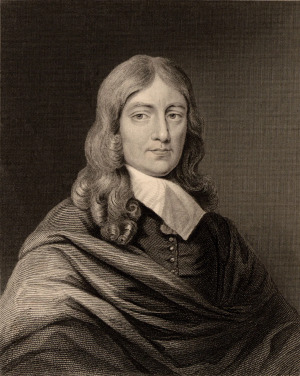
\includegraphics[scale=0.25]{milton}
		\caption{John Milton}
	\end{figure}%
	\begin{figure}
		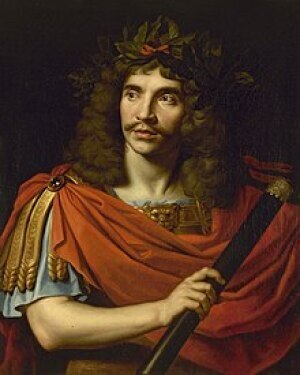
\includegraphics[scale=0.25]{molier}
		\caption{Molière}
	\end{figure}

	\end{columns}
\end{frame}
\begin{frame}

\frametitle{18. storočie}
\subsection{18. storočie}
\begin{itemize}
	\item Literatúra ovplyvnená osvietenstvom
	\item Vznik moderného románu
	\item Encyklopédia
\end{itemize}
\begin{minipage}[t]{0.5\textwidth}
	\kern0pt
	\begin{figure}
		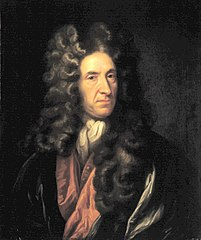
\includegraphics[scale=0.4]{defoe}
		\caption{Daniel Defoe}
	\end{figure}
\end{minipage}%
\begin{minipage}[t]{0.5\textwidth}
	\kern0pt
	\begin{figure}
		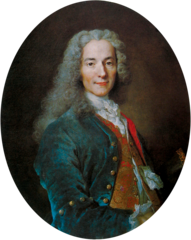
\includegraphics[scale=0.4]{voltik}
		\caption{Voltaire}
	\end{figure}
\end{minipage}


\end{frame}

\begin{frame}{\small{18. storočie} / \Large Významní spisovatelia 18. storočia}
	
\subsubsection{Významní spisovatelia 18. storočia}
\begin{columns}
	
\column{0.6\textwidth}
\begin{itemize}
	\item Jonathan Swift
	\bigskip
	\item J.W. von Goethe
	\bigskip
	\item Denis Diderot
	\bigskip
	\item J.J. Rosseau
\end{itemize}
\column{0.4\textwidth}
	\begin{figure}
		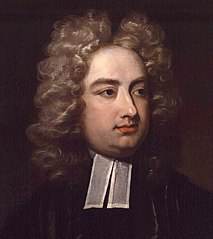
\includegraphics[scale=0.4]{swift}
		\caption{Jonathan Swift}
	\end{figure}%
	\begin{figure}
		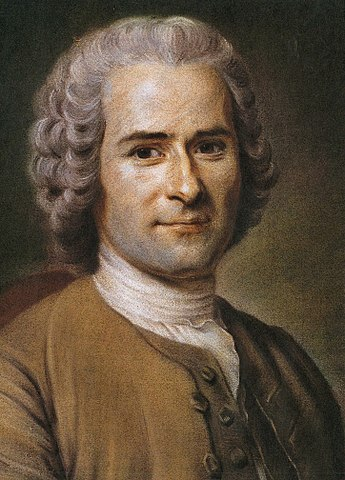
\includegraphics[scale=0.225]{rosseau}
		\caption{J.J. Rosseau}
	\end{figure}

	\end{columns}
\end{frame}


\section{Architektúra}
\frame{\sectionpage}
\begin{frame}{Baroková architektúra}
	\subsection{Baroková architektúra}
	\begin{itemize}
		\item Barok - nepochopený smer
		\item Vznikol na začiatku 17. storočia v Taliansku
		\item Dekoratívne prvky - podpora katolíkov
	\end{itemize}
		\begin{columns}
		\column{0.8\textwidth}
		\begin{figure}
			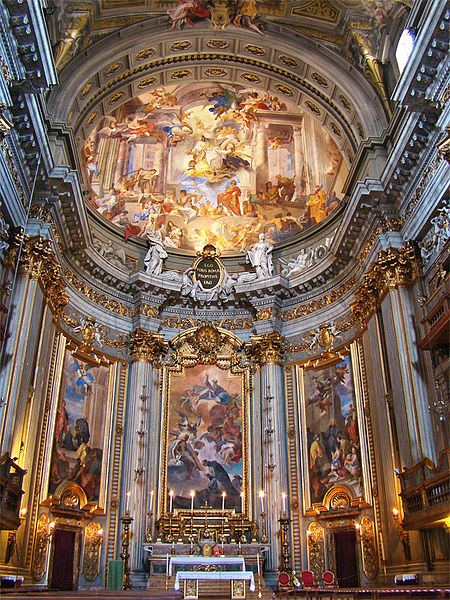
\includegraphics[scale=0.35]{loyola}
			\caption{Interiér kostola sv. Ignáca z Loyoly, Rím}
		\end{figure}
		\column{0.2\textwidth}
		\end{columns}
\end{frame}
\begin{frame}
	\frametitle{Zdroje}
	\section{Zdroje}
	\begin{itemize}
		\large \item KNIHY
		\begin{itemize}\tiny
			\item Evans, Benjamin Ifor, a Bergonzi, Bernard. A short history of English literature. Penguin books, 1940.
			\item Briggs, Martin Shaw. Baroque architecture. TF Unwin, 1913.
		\end{itemize}
		\large \item INTERNET
		\begin{itemize}
			\tiny
			\item   \url{https://www.britannica.com/art/Western-literature/The-17th-century}
			\item   \url{https://en.wikipedia.org/wiki/17th\_century\_in\_literature}
			\normalsize
		\end{itemize}
	\end{itemize}
\end{frame}
\end{document} 
